\documentclass[a4paper]{report}
%\documentclass[a4paper,twoside]{article}



\usepackage[utf8]{inputenc}
\usepackage[T1]{fontenc}
\usepackage{lmodern}
\usepackage[francais]{babel}
\usepackage[pdftex,bookmarks=true,bookmarksnumbered=true]{hyperref}
\usepackage{amsmath}
\usepackage{amsfonts}
\usepackage{amssymb}
\usepackage{algorithm,algorithmic}
\usepackage{float}
\usepackage{caption}
\usepackage{graphicx}
\usepackage{comment}

\usepackage[nottoc, notlof, notlot]{tocbibind}


\begin{document}
\tableofcontents
\chapter{Présentation des différentes méthodes}
\section{Hypothèses}
Durant tout ce chapitre les hypothèses suvantes seront prises en compte :\\
\begin{itemize}
  \item Il n'y a qu'un réservoir
  \item pour chaque turbine la fonction de production est linéaire par rapport au débit si le volume d'eau contenu dans le réservoir est fixé.
\end{itemize}
\section{Programmation linéaire}
\subsection{Principe}
\textbf{Fonction objective :}
\begin{center}
 $Max(\sum_t\sum_h\sum_i C_{t,i}\times PrixSpot_h \times x_{h,t,i})$
\end{center}
Avec\\
\begin{itemize}
\item $x_{h,t,i}$ : Quantité turbinée à l'heure $h$ avec la turbine $t$ si le volume du réservoir dans l'intervalle $i$, 0 sinon.
\item $C_{t,i}$ : Coefficient de productivité de la turbine $t$ si le réservoir contient un volume d'eau compris dans l'intervalle $i$. 
\item $PrixSpot_h$ : le prix spot à l'heure $h$.
 \end{itemize}
\textbf{Contraintes :}
\[\begin{aligned}
 \sum_i d_{h,t,i}&\leq1  &\forall h,t\ (1)\\
 V_{min}&\leq V_{h} -\sum_{p}\sum_{k<h}\sum_j x_{k,p,j} - \sum_{k<h} r_{k}& \forall h \ (2)\\
f_i. d_{h,t,i} + V_{max}(1-d_{h,t,i})&\geq V_{h} - \sum_{p}\sum_{k<h}\sum_j x_{k,p,j} - \sum_{k<h} r_{k}&\forall i,h,t\ (3)\\
C_{t,i} \frac{x_{h,t,i}}{3600}&\geq prodMin_t \times d_{h,t,i} & \forall i,h,t\ (4)\\
\frac{x_{h,t,i}}{3600} &\leq d_{h,t,i}\times q_{t,max} &\forall i,h,t\ (5)\\
\sum_{t}\sum_{h}\sum_{i} x_{h,t,i} +  \sum_{h} r_{h} &= Apports_{annee}- 8760 q_r  &(6)\\
x_{h,t,i}  &\geq 0 , d_{h,t,i}  \in \{0,1\}  & \forall h,t,i\ (8)
\end{aligned}\]
Avec :\\
\begin{itemize}
\item $d_{h,t,i}$ : Une variable binaire qui vaut 1 si on décide d'utiliser la turbine $t$ à l'heure $h$ et que le volume du réservoir est compris dans l'intervalle $i$ à l'heure $h$, 0 sinon.
\item $r_h$ : La quantité d'eau qui est déversée à l'heure $h$ sans être turbinée en plus de l'eau réservée.
\item $V_{h}= V_{init}+\sum_{i< h} apports_i - reserve\times (h-1)$
\item $f_i$ : la borne supérieure de l'intervalle $i$.
\item $Apports_{annee}$ : La quantité totale d'eau apportée au réservoir au cours de l'année.



\end{itemize}

\textbf{Explications}
\begin{itemize}
\item Les contraintes (1) et (3) permettent que $d_{h,t,i}$ soit nul si le réservoir ne se trouve pas dans l'intervalle $i$ à l'heure $h$. On use du fait de la croissance des coefficients de productivité
avec le volume pour s'assurer du respect de la borne inférieure de l'intervalle $i$ (qui est égale à la borne supérieure de l(intervalle $i-1$).
\item Les contraintes (2) assurent le respect de la contrainte de capacité minimale du réservoir.
\item Les contraintes (4) assurent le respect des contraintes de productivité minimale
\item Les contraintes (5) assurent le respect des contraintes de débit maximal et que $x_{h,t,}$ soit nul si $d_{h,t,i}$ est nul. 
\item La contrainte (6) permet d'assurer que tous les apports soient évacués à la fin de l'année.

\end{itemize}

\subsection{Résultats}
Le tableau ci dessous présente une étude statistique des temps de calculs necessaire en seceondes pour obtenir une solution optimale pour une planificatiojn sur 24h puis sur une semaine. Pour obtenir ses résultats nous avons à chaque fois tester 20 scénarios en faisans varier les apports.\\
\begin{tabular}{|l|c|l|}
  \hline
  &Sur une journée&Sur une semaine\\
  \hline
  Min &0.3690 &515.0\\
  \hline
  1er qu & 0.9175&649.7  
\\
  \hline
  Mediane & 0.9840&782.3  
\\
  \hline
  Moyenne &1.1266 & 816.9  
\\
  \hline
  3eme Qu &1.2075&972.9\\
  \hline
  Max & 3.4110 &1193.5\\

 
  \hline
\end{tabular}
\\
\subsection{Idées et perspectives}
\section{Programmation dynamique}
\subsection{Principe}
Les algorithmes de programmation dynamique on était introduit par Belman \cite{dynaRef}.\\
L'idée de l'algorithme est de construire un arbre dont chaque sommet représente un état possible du réservoir à une date t, c'est à dire
dont chaque sommet donne le
volume d'eau contenu dans le réservoir à un instant t. On discrétise les quantités d'eau à débiter et on a donc un nombre fini d'états 
possibles . \\
On crée un arc entre deux sommets s'il est possible de passer de l'état initial de l'arc à l'état final de l'arc en débitant une 
certaine quantité d'eau $q$ du réservoir. Les arcs sont évaluer par le profit maximal que l'on peut faire en débitant la quantité
$q$ du réservoir à l'heure associé au sommet final de l'arc sachant que le réservoir contient le volume d'eau associé au sommet initial de
l'arc.\\
Une fois le graphe créé on utilise l'algorithme de Belman pour trouver le plus long chemin entre le sommet représentant l'état initial
du système et celui représentant l'état final.


 \begin{center}
 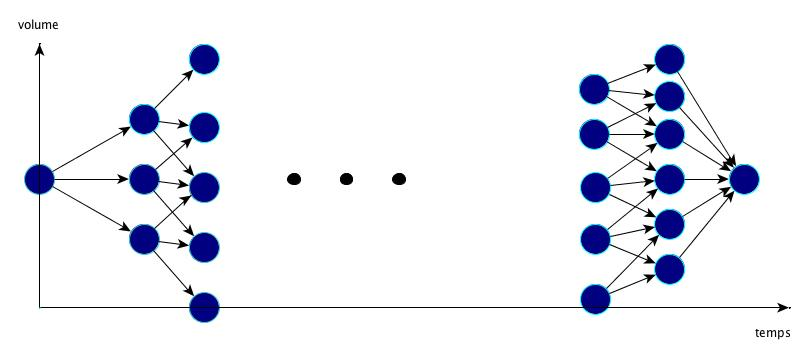
\includegraphics[scale=0.5]{images/dynamique.jpg}
 \end{center}
\subsubsection*{Création des sommets}
On va essayer de réduire la taille du graphe au maximum. Pour cela on peut tout d'abord remarquer qu'il n'y aura jamais intérêt à débiter
sans turbiner à moins que e soit pour respecter la contrainte de volume maximum du fait de la croissance des coefficients de productivité avec le volume.\\
Par contre il est maintenant possible qu'une solution pour laquelle on débite de l'eau sans la turbiner pour respecter la contrainte de
volume maximale, permette d'obtenir un plus grand profit qu'une ou toute l'eau en surplus serait turbinée avant l'heure critique.\\
On va réduire la création de sommets à ceux correspondant à des états qui sont atteignables uniquement en débitant des quantités d'eau
turbinables ou qui correspondent au volume maximum.
\subsubsection*{Création des arcs}
On crée un arc entre deux sommets  $s_1$ et $s_2$ si $heure(s_2)=heure(s_1)+1 $et :
\begin{center}
 $k_{min} \leq q \leq k_{max}$ \\
OU\\
$q > 0$ et $ volume(s_2)=V_{max}$
\end{center}
Avec :\\
\begin{itemize}
\item $h=heure(s_1)$
\item $q = volume(s_1)+ Apport_{h+1} - reserve -volume(s_2)$
\item $k_{min}= min_t(prodMin_t/C_{t,i})$ \\
Avec $i$ l'intervalle dans lequel se trouve $volume(s_1)$ 
\item $k_{max}= \sum_t q_{max,t}$

 
\end{itemize}
\subsubsection*{Evaluation des arcs}
Comme nous l'avons vu précédemment le problème de l'évaluation des arcs est NP-Complet, en effet il s'agit du problème restreint à une planification sur une unique période. Nous avons proposé deux approches pour ce problème, une approche exacte en utilisant un solveur pour résoudre un programme linéaire en variables mixtes, et une approche approchée avec un algorithme glouton.
\subsubsection*{Évaluation exacte}
On peut pour avoir une évaluation exacte de nos arcs, utiliser cplex pour résoudre le programme linéaire en variables mixtes suivant :\\

\begin{center}
 $Max(\sum_t C_{t}\times PrixSpot \times x_{t})$
\end{center}
\[\begin{aligned}
\sum_{t} x_{t} + r &= q &\quad (1)\\
x_{t}  &\leq d_{t}\times q_{t,max} &\forall t\quad(2)\\
x_{t}  &\geq  d_{t}\times q_{t,min}  & \forall t\quad(3)\\
d_{t}  &\in \{0,1\}  & \forall t\quad(4)\\
r  &\geq 0  & \quad(5)
\end{aligned}\]
Avec :\\
\begin{itemize}
\item $C_{t}$ : le coefficient de productivité de la turbine $t$ sachant que le volume du réservoir est celui du sommet initial de l'arc à évaluer.
\item $PrixSpot$ : le prix sport à l'heure correspondant au sommet final de l'arc à évaluer.
\item $x_t$: variable réelle représentant la quantité d'eau débitée pour la turbine t.
\item $r$ : la quantité d'eau débitée sans être turbinée.
\item $q$ : la quantité d'eau qu'il faut débiter pour pouvoir passer de l'état initial de l'arc à l'état final de l'arc.
\item $d_t$ : variable binaire qui vaut 1 si l'on décide d'utiliser la turbine $t$, 0 sinon.
\item $q_{min,t}$ : quantité minimale d'eau qu'il faut débiter avec la turbine $t$ pour respecter sa contrainte de production minimale.
\end{itemize}
\subsubsection*{Évaluation gloutonne des arcs}
Le principe de l'évaluation gloutonne des arcs est le suivant :\\
\begin{itemize}
\item Classer les turbines par ordre décroissant suivant leur coefficient de productivité.

\item Pour chaque turbine de la liste triée lui associer le maximum d'eau possible jusqu’à'à ce que toute l'eau soit distribuée.
\end{itemize}
Cette évaluation à l'avantage de nous permettre d'avoir un algorithme pseudo polynomial, puisque le coût de notre algorithme de programmation dynamique est dès lors en  O($\frac{kmax}{pas}^{2}\times nbHeures^{4}$).\\
Néanmoins cette approximation est très mauvaise, elle ne fournit aucune garantie de performance , nous allons en effet montrer que quelque soit l'écart $e$ , il existe des instances $I$ du problème (dévaluation des arcs) pour lesquelles on ait :\\
\begin{center}
$ s_{opt}(I)-s_{G}(I)\geq e$
\end{center}
En effet si on considère l'instance I suivante :\\
\begin{itemize}
\item $nbTurbines \longleftarrow 2$
\item $q \longleftarrow e+2$
\item $q_{max,1}\longleftarrow1$
\item $q_{min,1}\longleftarrow0$
\item $C_1\longleftarrow 2$
\item $q_{max,2}\longleftarrow q$
\item $q_{min,2}\longleftarrow q$
\item $C_2\longleftarrow 1$
\end{itemize}
L'algorithme glouton donne une solution égale à 2 alors que l'optimal est égal à $e+2$.\\
Néanmoins sur nos jeux de donnés l'écart n'est en moyenne que de 2.703437 $\%$ avec un écart type de 2.116533 $\%$.
\subsection{Résultats avec évaluation gloutonne}
Le tableau ci dessous présente une étude statistique des temps de calculs necessaire en seceondes pour obtenir une solution optimale pour une planificatiojn sur 24h puis sur une semaine. Pour obtenir ses résultats nous avons à chaque fois tester 10 scénarios en faisans varier les apports.\\
\begin{tabular}{|l|c|l|}
  \hline
  &Sur une journée&Sur une semaine\\
  \hline
  Min &0.279 &964.2\\
  \hline
  1er qu & 0.676&1119.7 
\\
  \hline
  Mediane & 1.242&1356.4 
\\
  \hline
  Moyenne &1.366 & 1293.5
\\
  \hline
  3eme Qu &1.970&1430.8\\
  \hline
  Max & 2.619 &1577.0\\
\hline
 ecart type & 0.841734 & 209.3559\\
 
  \hline
\end{tabular}
\\
\subsection{Améliorations}
L'idée d'amélioration se base sur l'observation du fait que si l'on considére deux sommets quelconques du graphes, s'il existe des chemins les reliants, ceux ci possèdent tous le même nombre d'arcs. Ainsi on peut construire la solution itérativement de la maniere suivante :\\
\subsubsection*{Création des sommets}
Lors de la création des sommets on leur associe à chacun un poids égale à moins l'infini, sauf pour le sommet racine auquel on associe un poids nul . Ce poids représentera la valeur du plus long chemin entre le sommet racine et le sommet valué.\\
\subsubsection*{Création des arcs}
A prrèsent à chaque sommet $s$ d'heure $h$ on n'associe qu'un seul et unique prédécesseur de la façon suivante: \\

 \begin{algorithm}[H]
 \caption{Construction des arcs}
 
 
 \begin{algorithmic}


 \FOR {tout les sommet $s'$ tels que l'on puisse passer de l'état associé à $s'$ à celui associé à $s$}
 \IF{ poids($s'$)+eval($s,s'$)>poids($s$)}
 \STATE poids($s$)$\longleftarrow$ poids($s'$)+eval($s,s'$)
\STATE pred($s$)$\longleftarrow s'$
 \ENDIF

 \ENDFOR
 

 \end{algorithmic}
 \end{algorithm}
Où la fonction eval(sommet,sommet) est une fonction permettant d'évaluer les arcs, soit par la méthode exacte, soit par la méthode gloutonne.\\

Ainsi, on n'a plus besoin d'appliquer l'algorithme de Belmann mais l'on peut simplement parcourir le chemin en partant du sommet final. Ce qui permet de passer d'une compléxité algorithmique en $O(nbHeure^4)$ à une complexité algorithmique en $O(nbHeure^2)$.
\subsubsection*{Remarque}
Cette méthode peut etre mise en oeuvre pour tout système dynamique pour lequel le nombre d'état par lesquels il faut passer pour aller d'un état donné à un autre est fixe.
\subsubsection*{Autre amélioration } Une autre idée d'amélioration est, afin de réduire le nombre d'évaluations, de considérer les sommets $s'$ associés à l'heure $h-1$ dans l'ordre croissant en fonction de la quantité d'eau distribuée jusqu'à l'heure $h-1$ associée. On s'appuie alors sur le fait que la fonction eval($s',s$) décroie quand la quantité associé à $s'$ croie (puisque des lors la quantité à débiter pour passer de $s'$ à $s$ décroie), et on se sert de cette observation pour réduire le nombre d'évaluation de la maniere suivante :\\
 \begin{algorithm}[H]
 \caption{Construction des arcs}
 
 
 \begin{algorithmic}

\STATE $derniereEval \longleftarrow 0$
 \FOR {tout les sommet $s'$ classés tels que l'on puisse passer de l'état associé à $s'$ à celui associé à $s$}
\IF{ poids($s'$)+derniereEval>poids($s$)}
\STATE $eval\longleftarrow eval(s',s)$
 \IF{ poids($s'$)+eval>poids($s$)}
 \STATE poids($s$)$\longleftarrow$ poids($s'$)+eval
\STATE pred($s$)$\longleftarrow s'$
\STATE $derniereEval\longleftarrow eval$
 \ENDIF
\ENDIF

 \ENDFOR

 

 \end{algorithmic}
 \end{algorithm}
Qui plus est la manière dont on crait les sommet fait qu'ils sont dirrectement bien classé, il n' y a donc pas à utiliser d'algorithme de tri.\\
\subsection{Résultats avec évaluation gloutonne}
Le tableau ci dessous présente une étude statistique des temps de calculs necessaire en seceondes pour obtenir une solution optimale pour une planificatiojn sur 24h, une semaine, un mois puis un an. Pour obtenir ses résultats nous avons à chaque fois tester 10 scénarios en faisans varier les apports.\\
\begin{tabular}{|l|c|c|l|}
  \hline
  &Sur une journée&Sur un mois&Sur un an\\
  \hline
  Min &0.08200 &1.585&26.63\\
  \hline
  1er qu & 0.08325 & 1.639 &30.59
\\
  \hline
  Mediane & 0.08600&1.736 &36.42
\\
  \hline
  Moyenne &0.08550 & 2.009 &39.89
\\
  \hline
  3eme Qu &0.08675&2.114&40.83\\
  \hline
  Max & 0.08900 &3.257&80.33\\
\hline
 ecart type & 0.002460804 & 0.5551685 &16.44358\\
 
  \hline
\end{tabular}
\\
\subsection{Résultats avec évaluation exacte}
Le tableau ci dessous présente une étude statistique des temps de calculs necessaire en seceondes pour obtenir une solution optimale pour une planificatiojn sur 24h, une semaine, un mois puis un an. Pour obtenir ses résultats nous avons à chaque fois tester 20 scénarios en faisans varier les apports.\\
\begin{tabular}{|l|c|c|l|}
  \hline
  &Sur une journée&Sur une semaine &Sur un mois\\
  \hline
  Min &10.76 &1042&4336\\
  \hline
  1er qu & 22.70 & 1117   &4862
\\
  \hline
  Mediane & 33.41&1174 &4907
\\
  \hline
  Moyenne &31.29 & 1310 &5390  

\\
  \hline
  3eme Qu &38.13&1430&6253\\
  \hline
  Max & 47.55 &1899&6566\\
\hline
 ecart type &291.3738 & 0.5551685 &886.338\\
 
  \hline
\end{tabular}
\\
\subsection{Cas une turbine}
Dans le cas où il n'y a qu'une turbine, alors l'évaluation des arcs est triviale, car elle correspond simplement calculer le profit obtenu en débitant la quantité à débiter pour passer de l'état représenté par le sommet initial de l'arc  à celui représenté par le sommet final.
Dans ce cas l'algorithme a une compléxité psseudo polynomiale , son coût au pire des des cas est en :\\
\begin{center}
   O($\frac{kmax}{pas}^{2}\times nbHeures^{4}$)
\end{center}
\subsubsection{Résultats}
Le tableau ci dessous présente une étude statistique des temps de calculs necessaire en seceondes pour obtenir une solution optimale pour une planificatiojn sur 24h, une semaine, un mois puis un an. Pour obtenir ses résultats nous avons à chaque fois tester 20 scénarios en faisans varier les apports.\\
\begin{tabular}{|l|c|l|}
  \hline
  &Sur une semaine &Sur un an\\
  \hline
  Min &0.2260&15.42\\
  \hline
  1er qu & 0.2450 & 22.31
\\
  \hline
  Mediane & 0.2525&28.91
\\
  \hline
  Moyenne &0.3399 & 58.67 

\\
  \hline
  3eme Qu &0.2777&70.05\\
  \hline
  Max & 1.0130 &215.52\\
\hline
 ecart type &0.2407255 &61.64453 
\\
 
  \hline
\end{tabular}
\subsection{Cas deux turbines}
Dans le cas où il n' y a que deux turbines, on restreint les appels à cplex pour l'évaluation des arcs aux cas où l'on est pas dans l'une des configurations suivantes :\\
soit q la quantité à déverser pour paser du sommet initiale au sommet final, h l'heure à laquelle on déverse, i l'intervalle correspondant au volume associé au sommet initial de l'arc.\\
On suppose que la turbine pour laquelle le coefficient de productivité est le plus grand est la turbine 1. $q_{max,t}$ et $q_{min,t}$ correspondent respéctivement à la quantité maximale et à la quantité minimale que l'on peut déverser avec la turbine $t$ sachant que le reservoir se trouve dans l'intervalle $i$.\\
$w_t$ représente le coefficient de productivité de la turbine $t$ sachant que le volume contenu dans le réservoir se situe dans l'intervalle $i$ et $prixSpot_h$ le prix spot à l'heure $h$.\\
\begin{itemize}
  \item Si ($q_{min,1}\leq q \leq q_{max,1}$)\\
  \subitem Alors $eval = w_1 \times prixSpot_h \times q$\\
  \item Si ( $q\geq q_{max,1}+q_{min,2}$)\\
  \subitem Alors $eval=(w_1 \times q_{max,1} + w_2 \times min(q- q_{max,1},q_{max,2}))$\\
  \item Si ( $q_{min,2}\leq q  < q_{min,2}$)\\
  \subitem  Alors $eval= w_2 \times min(q,q_{max,2})$
\end{itemize}
\subsubsection{Résultats}
Le tableau ci dessous présente une étude statistique des temps de calculs necessaire en seceondes pour obtenir une solution optimale pour une planificatiojn sur 24h puis sur une semaine. Pour obtenir ses résultats nous avons à chaque fois tester 10 scénarios en faisans varier les apports.\\
\begin{tabular}{|l|c|c|l|}
  \hline
  &Sur une journée&Sur une semaine&Sur un mois\\
  \hline
  Min &1.872 &95.66 & 541.7\\
  \hline
  1er qu & 2.621&122.02 & 620.9
\\
  \hline
  Mediane & 3.434&140.90 & 752.6
\\
  \hline
  Moyenne &3.403& 136.87 & 725.1
\\
  \hline
  3eme Qu &3.985&152.56 & 800.9\\
  \hline
  Max & 4.928 &169.63 &940.7\\
\hline
 ecart type &1.018996 & 23.50096 & 135.3985\\
 
  \hline
\end{tabular}
\\
\subsection{Résultats}
\section{Hybridation algorithme génetique méthode exacte par décompostion spaciale}
\subsection{Principe}
\subsubsection{Idée}
\begin{center}
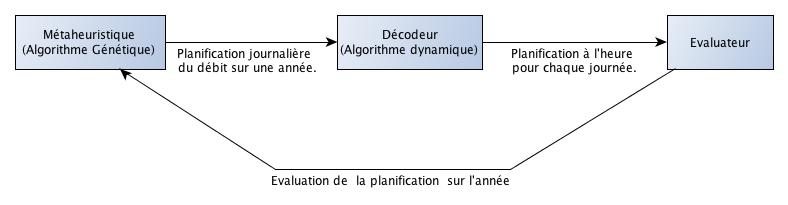
\includegraphics[scale=0.5]{images/interactionModules.jpg}
\end{center}
L'idée est d'utiliser une métaheuristique qui permette de distribuer la quantité totale d'eau à évacuer durant l'année entre les différents jours de cette année.  La métaheuristique manipule donc un calandrier au jour le jour des débits effectués sur le réservoir. Pour passer de cette représentation journalière des débit à une représentation donnant le débit effectué pour chaque turbine et conduite heure par heure, on utilise un décodeur qui est soit l'algorithme génétique avec évaluation gloutonne soit le MIP.\\
Le décodeur nous permettra également d'obtenir une évaluation des solutions fournies par la métaheuristique, évaluation qui sera elle même réutilisée dans la métaheuristique.\\

\subsubsection{L'algorithme génétique}
Pour notre métaheuristique nous avons choisi d'utiliser l'algorithme génétique. Nous allons donc tout d'abord expliquer ce qu'est un algorithme génétique :\\
\begin{center}
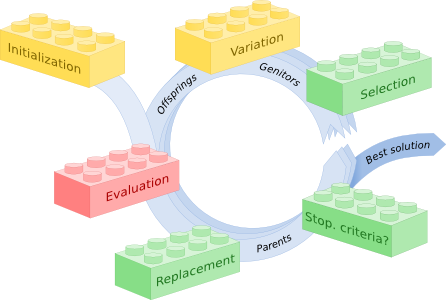
\includegraphics[scale=0.5]{images/Evolutionary_algorithm}

\end{center}
Un algorithme génétique est un algorithme qui se base sur les idées de la 
théorie de l'évolution de l'espèce pour résoudre des problèmes . L'idée est de construire une population de base, dont chaque individu représente une solution réalisable du problème . Cette population doit être la plus diversifiée possible, en générale elle est initialisée aléatoirement. On attribue à chaque individu une note qui correspond  pour un problème d'optimisation à la valeur de la fonction objective pour la solution correspondante, cette note représente en termes biologiques, le fait qu'un individu soit plus ou moins adapté à son environnement.\\
On effectue ensuite une sélection au sein de la population, la sélection peut se faire de plusieurs manières, mais dans notre cas nous ferons une sélection aléatoire proportionnelle au niveau d'adaptation de chaque individu, c'est à dire que les individus les plus adaptés auront le plus de chance d'être sélectionnés.  Lorsque deux individus (ou chromosomes) sont sélectionnes on leur applique avec une certaine probabilité un opérateur de croisement, opérateur qui permettra de générer des solutions "filles" à partir de ses deux solutions, c'est à dire des solutions dans lesquelles des caractéristiques des deux parents se retrouvent. Puis avec une très faible probabilité un opérateur de mutation qui doit permettre de diversifier l'ensemble des solutions.\\
En effectuant ces opérations (croisement, mutation) un certain nombre de fois , on se retrouve alors avec une nouvelle population (la première génération) ayant la même taille que la population initiale, et qui contient globalement des solutions plus proches de l'optimum. Le principe des algorithmes génétiques est d'effectuer ces opérations un maximum de fois de façon à augmenter la justesse du résultat. En général le critère d'arrêt est un nombre de générations, ce sera le cas pour nous.\\
Pour définir notre algorithme génétique nous avons donc à définir : \\
\begin{itemize}
\item la représentation de nos individus
\item l'initialisation
\item l'opérateur de mutation
\item l'opérateur de croisement
\item l'évaluation
\end{itemize}
\subsubsection{La représentation}
\begin{center}
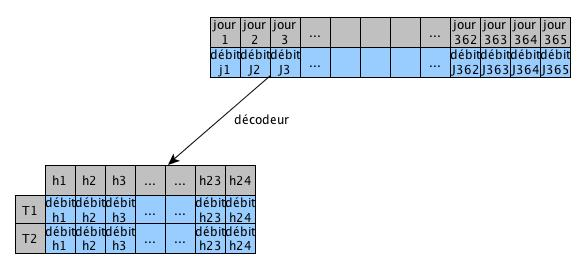
\includegraphics[scale=0.6]{images/representation.jpg}
\end{center}
La représentation se fera sous forme d'un tableau de 365 cases qui donnera pour chaque jour la quantité totale d'eau débitée du réservoir (en plus de l'eau réservée automatiquement).\\
Pour qu'une solution soit valide il faut :\\
\begin{itemize}
\item Que la somme des débits journaliers soit égale à la quantité à débiter sur l'année.
\item Que les quantités débitées avant un jour donné soit suffisante pour permettre le respect de la contrainte de volume maximal.
\item Que les quantités débitées avant un jour donné n'entrainent pas l'impossibilité de respecter la contrainte de volume minimal sur ce jour.
\end{itemize}
Néanmoins dans la pratique nous ne nous soucierons pas de la dernière contrainte quand nous appliquerons nos opérateurs, car celle ci sera corrigée dans le décodeur, qui reportera les quantités d'eau à débiter en excé sur un jour au jour suivant.\\
Le décodeur nous permet de passer à une représentation donnant pour chaque heure le débit à effectuer pour chaque turbine. Le décodeur utilisera aléatoirement l'algorithme dynamique avec évaluation gloutonne des arcs ou le programme linéaire en variables mixtes. Mais avec une plus forte probabilité pour l'algorithme dynamique car celui ci est moins coûteux en terme de temps de calcul.\\
\subsubsection{L'initialisation}
On va chercher à générer une population de solutions qui soient réalisables, c'est à dire qui
permettent d'éviter un débordement du réservoir,
et donc qui vérifient l'inégalité suivante :\\
\begin{center}
$q^{s}\geq V^{s}_{init}+ A^{s}-V_{max}- qr\times 168\quad (1)$ 
\end{center}
Avec:\\
\begin{itemize}
\item $q^{j}$ : quantité d'eau débitée lors de la journée j.
\item $V^{j}_{init}$ : volume d'eau contenu dans le réservoir en début de journée.
\item $A^{j}$ : quantité totale d'eau apportée  lors de la journée j.
\item $V_{max}$: Capacité maximale du réservoir.
\item $qr \times 24$ : quantité totale d'eau réservée automatiquement en une journée.
\end{itemize}
On a de plus :\\
\begin{center}
$V^{j}_{init}=V_{init} +\sum_{i<j}A^{i}-\sum_{i<j}q^{i} - (j-1) q_{r}$
\end{center}
Où $V_{init}$ est la quantité d'eau contenue dans le réservoir en début d'année.\\

On va chercher de plus à ce que la quantité d'eau donnée puisse être débitée entièrement, c'est à dire à ce que l'on ne débite pas plus d'eau que ce que le réservoir en contient. Pour cela on ajoute la contrainte suivante : \\
\begin{center}
$q^s \leq V^{s}_{init}+ A^{s}- qr \times 168 \quad(2) $
\end{center}
On peut faire un algorithme d'initialisation aléatoire itératif permettant de
distribuer la quantité souhaitée ( apport total annuel) sur toutes les semaines de
manière à respecter les contraintes énoncées ci dessus.\\
On peut aussi réutiliser le principe de l'algorithme présenté pour la résolution du premier cas mais en remplaçant la distribution gloutonne des débits par une distribution aléatoire de ceux ci.
C'est à dire :\\
\begin{itemize}
\item Rechercher la première Journée à laquelle il y aurait excès d'eau si on ne déversait pas.
\item Appliquer un algorithme aléatoire pour trouver la planification  des débits permettant de déverser la quantité en excès avant la journée critique en respectant les contraintes énoncées ci dessus et également la contraintes de ne pas débiter plus d'eau qu'on ne peut en turbiner si ce n'est pour la journée critique .

\item Pour les jours $j$ suivantes appliquer l'algorithme glouton pour débiter avant le jour $j$ la nouvelle quantité excédante, en considérant les débits déjà planifiés.
\item Utiliser une dernière fois l'algorithme de distribution pour trouver la façon optimale de déverser la quantité restant à déverser pour respecter la contrainte d'évacuation totale.
\end{itemize}
Cette méthode d'initialisation permet d'accélérer la convergence de l'algorithme car elle permet de partir d'une population de base qui tout en étant meilleure reste variée.
\subsubsection{La mutation}
L'opération de mutation consiste à  transvaser  une parti de l'eau débitée du réservoir à la date j (choisie au hasard) dans la quantité d'eau débitée du réservoir à la date j' (choisie au hasard).
La quantité d'eau à transvaser sera choisie aléatoirement mais de manière à ce que le fait d'enlever cette quantité de la quantité à débiter du réservoir à la date j ne provoque pas de débordement de celui ci.  Pour ce faire on impose une contrainte de borne :\\

Notons:\\
\begin{center}
$q_{n}^{s}=V^{s}_{init}+ A^{s}-V_{max}- q_{r}$
\end{center}
$q_n^s$ représente la quantité qui déborderait du réservoir s'il n'y avait pas d'eau débitée.\\
Pour que le réservoir ne déborde pas (condition (1)), si $s_{1}$ et $s_{2}$ correspondent aux deux points sélectionnés pour effectuer la mutation:\\
\begin{itemize}
\item $j_{1}$ : Journée à laquelle on retire une quantité $q_{t}$ d'eau.
\item $j_{2}$ : Journée laquelle on ajoute une quantité $q_{t}$ d'eau.
\end{itemize}
 Il y a alors deux possibilités, soit $ j_{1} < j_{2}$ :\\
 Dans ce cas pour tous les jours j compris entre $j_{1}$ et $j_{2}$ on a :\\
 \begin{center}
$V^{j}_{m,init}=V_{init} +\sum_{i<j}A^{i}-\sum_{i<j}q^{i}  +q_{t} - (j-1) q_{r} = V^{j}_{init}+ q_{t}$
\end{center}
où $V^{j}_{m,init}$ représente la quantité initiale dans le réservoir pour la journée j après mutation.
Pour que la condition (1) soit vérifiée il faudra donc que :\\
\begin{center}
$q_{t}\leq q^{j}-q^{j}_{n} \quad \forall j, j_{1}\leq j< j_{2}$
\end{center}
La condition (2) est elle toujours vérifiée puisque étant donné que l'on ne débite pas la quantité $q^t$ d'eau la semaine $j_1$ celle ci sera disponible à la date $j_2$. Donc dans la mesure ou cette condition était vérifiée avant la mutation elle le sera toujours après.\\
Soit $ j_{1} > j_{2}$ :\\
Dans ce cas pour toute semaine s comprise entre $s_{2}$ et $s_{1}$ on a :\\
 \begin{center}
$V^{s}_{m,init}=V_{init} +\sum_{i<s}A^{i}-\sum_{i<s}q^{i}  -q_{t} - (s-1) q_{r} = V^{s}_{init}- q_{t}$
\end{center}
et alors le nouveau volume initial étant plus petit, la condition (1) est toujours vérifiée. \\
En revanche la condition (2) peut poser problème, il faudra donc que :
\begin{center}
$q_t \leq V^j_{init} - q^j$
\end{center}
Remarque : En dehors de l'intervalle $[j_{1},j_{2}[$ ou $[j_{2},j_{1}[$ le volume initiale après mutation est le même que celui avant mutation et (1) est donc vérifiée.

\begin{center}
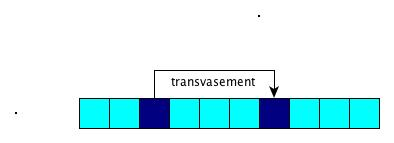
\includegraphics[scale=0.7]{images/mutation.jpg}
\end{center}
\subsubsection{Croisement}
Pour simplifier nous allons d'abord considérer un croisement en un point.
 \begin{center}
 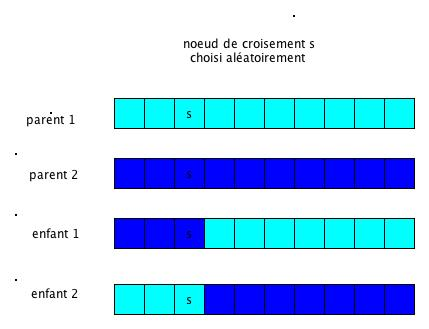
\includegraphics[scale=0.7]{images/croisement1pt.jpg}
 \end{center}
 la journée s est la journée de recoupement.  Posons: 
 \begin{itemize}
 \item $q_{p_{i},j}$ la quantité débitée la $j^{ieme}$ journée pour le parent $p_i$.
   \item $q_{p_{i}}=\sum_{j=0..51}q_{p_{i},j}=Q$
 \item $q_{p_{i},A}=\sum_{j=0..s}q_{p_{i},j}$
  \item $q_{p_{i},B}=\sum_{j=s+1..51}q_{p_{i},j}=Q-q_{p_{i},A}$\\
 \end{itemize}
 Où Q est égale à la somme des apports sur l'année.\\
A partir de deux parents $(p_{1})$ et $(p_{2 })$ on obtient deux enfant $e_{1}$ et $e_{2}$ de la manière suivante:\\
Si $q_{p_{1},A}> q_{p_{2},A}$ :\\
 \begin{itemize}
 \item $q_{e_{1},i}=q_{p_{1},i}\quad \forall i \in [[0,s]]$
  \item $q_{e_{1},i}=q_{p_{2},i}.\frac{q_{p_{1},B}}{q_{p_{2},B}}\quad \forall i \in [[s+1,365]]$\\
 \end{itemize}
 Si $q_{p_{1},A}<q_{p_{2},A}$ :\\
 \begin{itemize}
 \item $q_{e_{1},i}=q_{p_{1},i}.\frac{q_{p_{2},A}}{q_{p_{1},A}}\quad \forall i \in [[0,s]]$
  \item $q_{e_{1},i}=q_{p_{2},i}\quad \forall i \in [[s+1,365]]$\\
 \end{itemize}
  Si $q_{p_{1},A}=q_{p_{2},A}$ :\\
 \begin{itemize}
 \item $q_{e_{1},i}=q_{p_{1},i}\quad \forall i \in [[0,s]]$
  \item $q_{e_{1},i}=q_{p_{2},i}\quad \forall i \in [[s+1,365]]$\\
 \end{itemize}
 
 Pour obtenir $e_{2}$ on procède de la même manière en inversant les rôles de $p_{1}$ et $p_{2}$.\\
 La condition (2) ne sera pas toujours vérifiée lorsque $q_{p_{1},A}<q_{p_{2},A}$, mais le décodeur corrigera lui même ce genre de défaillance,l'eau qui n'aurait pas pu être débitée la semaine i étant débitée la semaine i+1. Montrons que les autres conditions sont vérifiées après croisement :\\
 \subsubsection*{On a $q_{e_{i}}=Q$ :}
 Une simple sommation des éléments mène au résultat en tenant compte du fait dans le cas d'égalité que  $q_{p_{i},B}=Q-q_{p_{i},A}$.\\
\subsubsection*{(1) est vérifiée :}
Le cas de $e_{2}$ étant identique, concentrons nous sur $e_{1}$.\\
 Si $q_{p_{1},A}> q_{p_{2},A}$ :\\
 Jusque s la condition  (1) est évidement vérifiée.\\
  Puis l'inégalité (1) peut se réécrire comme cela :\\
 \begin{center}
$\sum_{s\leq j <i}q_{p_{2},j}\geq V_{init} + \sum_{j\leq i}A_{j} - q_{p_{2},A} - q_{r}\quad \forall j \geq s \quad(2)$
 \end{center}
 On veut montrer que :\\
 \begin{center}
 $\sum_{s\leq j <i}q_{p_{2},j}.\frac{q_{p_{1},B}}{q_{p_{2},B}}\geq V_{init} + \sum_{j\leq i}A_{j} - q_{p_{1},A} - q_{r}$\\
 $=V_{init} + \sum_{j\leq i}A_{j} - q_{p_{2},A} - q_{r}-(q_{p_{1},A}-q_{p_{2},A})\quad \forall i \geq s$
 \end{center}

 On a  $q_{p_{1},B}<q_{p_{2},B}$, et donc $\frac{q_{p_{1},B}}{q_{p_{2},B}}<1$.  On peut écrire que:\\
 
 \begin{center}
 $q_{p_{2},j}.\frac{q_{p_{1},B}}{q_{p_{2},B}}= q_{p_{2},j}-a_{j}$
 \end{center}
 Avec:
 \begin{itemize}
 \item $a_{j}= q_{p_{2},j}- \frac{q_{p_{1},B}}{q_{p_{2},B}}. q_{p_{2},j}>0$
 \item$\sum_{j=s..51}a_{j}=q_{p_{2},B}-q_{p_{1},B}= q_{p_{1},A}-q_{p_{2},A}$
 \end{itemize}
 La véracité de l'inégalité précédente, partant de (2), est alors évidente.\\
  Si $q_{p_{1},A}<q_{p_{2},A}$ :\\
  Ce cas est simple puisque l'ajout de quantité d'eau dans la partie A du gène ne détériorera pas sa faisabilité vis à vis (1) et permettra de forcer la faisabilité de la partie  B du gène du fait que  dès lors :\\
  \begin{center}
  $V_{init,e_{1}}^{s}=V_{init,p_{2}}^{s}$
  \end{center}
\subsubsection{Évaluation}
L'évaluation s'effectue en appelant pour chaque journée le décodeur qui est soit avec un pourcentage $p$ le programme linéaire en variable mixte soit avec pourcentage $100-p$ l'algorithme dynamique avec évaluation gloutonne des arcs. Ce d'décodeur permet d'obtenir pour chacune des journées le profit maximal que l'on peut obtenir en déversant la quantité correspondante. On obtient une évaluation de l'individu en faisant la somme des différents profits journaliers.\\
Néanmoins cette évaluation reste très coûteuse pour un algorithme dynamique, en effet une évaluation pour une journée avec l'algorithme dynamique avec évaluation gloutonne des arcs prend en moyenne un peu plus de 1 seconde, donc pour évaluer un individu il faudrait en moyenne 365 secondes, soit plus de 6 minutes. Si on utilise le décodeur exacte, c'est à dire le programme linéaire en variables mixtes, il faut pour évaluer une journée en moyenne 2 secondes, donc pour évaluer un individu plus de 730 secondes.
\subsubsection{Valuation incrémentale}
Le principal inconvénient de cette méthode est la lenteur de la fonction d'évaluation, afin d'y remédier nous pouvons utiliser l'évaluation incrémentale.  Le principe est de ne réévaluer que les semaines sur lesquelles les transformation ( croisement et mutation) ont eu un impact. \\
Cet impact peut être lié à une modification du contenu initiale du réservoir, ou/ et à une modification de la quantité à distribuer.\\
Afin de mettre en place l'évaluation incrémentale il a fallu modifier la représentation pour pouvoir garder en mémoire l'évaluation de chaque journée et une indication quand à la validité de celle ci.
\subsubsection*{Après mutation}
Après une mutation seules les journées situées entre les deux points de déversement nécessitent une réévaluation. C'est à dire les semaines coloriées en vert sur la figure ci dessous :\\
\begin{center}
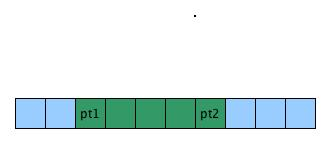
\includegraphics[scale=0.7]{images/deltaMutation.jpg}
\end{center} 
En effet la valeur des journées précédentes n'est pas modifiée, car ni les contenus initiaux des réservoirs ni les quantités à distribuer ne sont modifiées.\\
Les semaines suivantes ne sont pas modifiées non plus car les contenus initiaux sont identiques ( la quantité d'eau débitée avant ces semaines restant la même), et les quantités d'eau à distribuer ne sont pas modifiées non plus.\\
\subsubsection*{Tests }
Des tests unitaires sur 1000 individus on été effectués pour comparer la valeur de l'évaluation avec et sans delta évaluation après mutation, on obtient toujours le même résultat. Cela permet de valider l'implémentation de la nouvelle mutation et du décodage associé.\\
\subsubsection*{Après Croisement}

De même suite à un croisement il n'est pas nécessaire de réévaluer tous les jours.\\
Reprenons les trois cas précédemment expliqués :\\

Si $q_{p_{1},A}> q_{p_{2},A}$ :\\
On recalcule uniquement les valeurs des jours provenant du deuxième parent.\\
C'est à dire les jours encadrées en rouge sur le schéma ci dessous :\\
\begin{center}
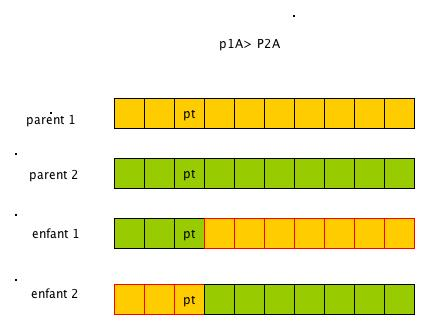
\includegraphics[scale=0.7]{images/deltaCroisement.jpg}
\end{center} 
 Si $q_{p_{1},A}<q_{p_{2},A}$ :\\
On recalcule uniquement les valeur des jours provenant du  premier parent.\\
  Si $q_{p_{1},A}=q_{p_{2},A}$ :\\
Les valeurs des jours ne sont pas à recalculer, il suffit de regarder quelle est la nouvelle somme pour obtenir la valeur de l'individu.\\
On se rend facilement compte de l'intérêt de l'évaluation incrémentale puisqu'on évaluera au maximum 365 jours au lieu de 730.

\subsection{Résultats}
\section{Hybridation algorithme génetique méthode exacte par décompostion spaciale avec représentation dynamique}`
\subsection{Principe}
Ce qui pose pas mal de problème dans la métaheuristique précédente, c'est que pour que l'individu soit valide il doit vérifier beaucoup de propriétés, ce qui fait que même pour appliquer nos opérateurs tres simples (croisement en un point et transvasement d'une quantité d'eau dans point à un autre) on a a effectuer des tests et des corrections. Ces corrections deviendraient encore plus complexes si l'on avait des opérateurs moins simple. Pour pallier à cette difficulté, nous avons décidé d'exploiter l'idée de représentation dynamique explicité dans l'article référencé en . L'idée est de donner la proportion d'eau débitée à une heure donnée par rapport à la quantité d'eau totale disponible à cette heure. 

\subsubsection*{Représentation}
On va représenter l'individu sous forme d'un tableau de $nbPeriode$ cases. 
Chaque case de ce tableau donne une proportion $p_t \in [0,1]$ d'eau à débiter durant une période $t$.\\
En fait si $V_{t-1}$ est le volume d'eau qui  est contenu dans le réservoir à la fin de la période $t-1 $ en effectuant les débit prévu par le tableau, alors la quantité $q_t$ d'eau à utiliser durant la période $t$ se calcul comme ceci :\\
 \begin{center}
   $q_{min}=max(0, V_{t-1}+Apport_t-reserve_t -V_{max})$\\
   $q_{dispo}=  V_{t-1}+Apport_t-reserve_t -q_{min} -V_{min}$\\
   $q_t= p_t \times q_{dispo}$
 \end{center}
 On ajoute une deuxième ligne au tableau qui contiendra la valeur de l'évaluation associée à chaque case pour la mise en place d'une évaluation incrémentale.
 \subsubsection*{Initialisation}
 \subsubsection*{Mutation}
 \subsubsection*{Croisement}
 \subsubsection*{Evaluation}
\subsection{Résultats}
\section{Programmation dynamique approximée utilisant un algorithme génétique}
Du fait de la taille du graphe qu'il m'anipule et du coût de l'évaluation d'un arc, l'algorithme dynamique dans sa première version est très couteux.  L'idée est donc d'utiliser une métaheuristique, ici un algorithme génétique, qui manipule directement les chemins dans ce graphe liant le sommet initial au sommet final.\\

\subsection{Principe}
\subsection*{Représentation}
Chaque individu représente un chemin du graphe de l'algorithme dynamique entre le sommet associé à l'état initail du sytème et le sommet associé l'état final du système. Par exemple un individu peut représenter le chemin rouge du graphe de l'algorithme dynamique ci dessous:
\begin{center}
  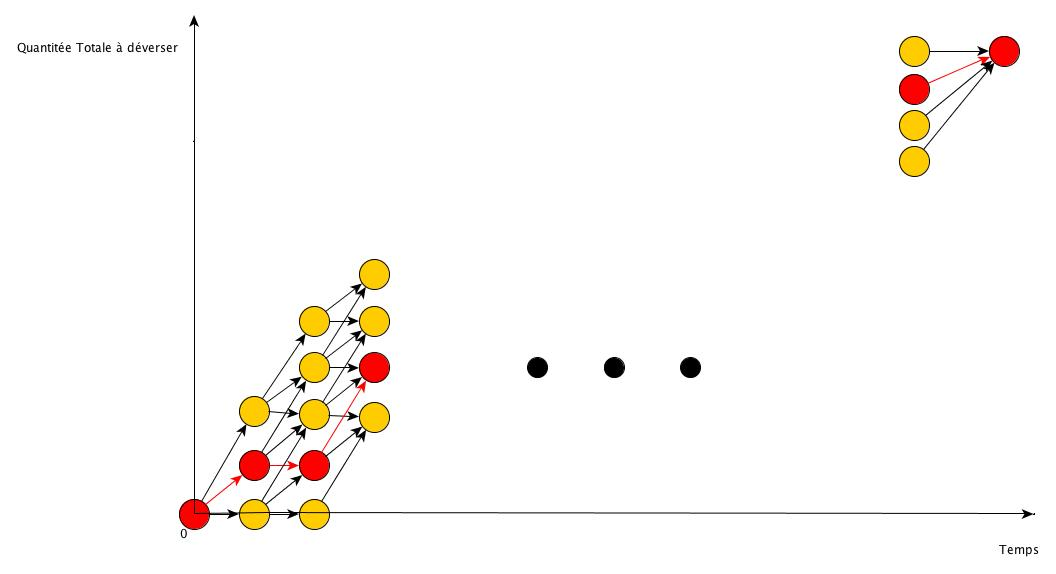
\includegraphics[scale=0.3]{images/grapheADG.jpg}
\end{center} 
Par contre on va choisir un arbre légérement moins restreint, l'explication de ce choix sera donnée ultérieurement. Les sommets correspondent au même sommets que ceux que l'on pouvait créer pour notre algorithme génétique mais on considere maintenant qu'il peut y avoir un arc entre deux sommets $s1$ et $s2$ à partir du moment où:\\
\begin{itemize}
\item $heure(s1)=heure(s2)-1$
\item $quantite(s1)\leq quantite(s2)$
\end{itemize}
Aussi le pas de discrétisation des quantités débitables n'est pas fixé, ce qui nous permetra d'obtenir eventuellement des solutions plus précises.\\
On représentera ses chemins sous forme d'un tableau où chaque case donnera pour une heure donnée la quantité d'eau qui a été débitée jusque cette heure. On obtient ensuite grace à un décodeur, la solution donnant la quantité d'eau à débitée pour chaque turbine à chaque heure ainsi que l'évaluation des arcs .\\

 \begin{center}
 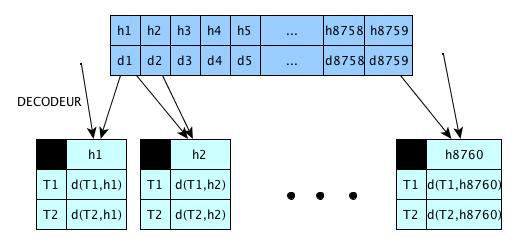
\includegraphics[scale=0.5]{images/representionADG.jpg}
 \end{center}
\subsection*{Initialisation}
L'initialisation s'effectue aléatoirement de façon incrémentale.
Pour chaque heure on choisit une quantité aléatoirement entre:
\begin{itemize}
  \item  $B_{min}=Max(V_h-V_{max},q_{h-1})$
  \item $B_{max}= Max(Min(V_h-V_{min},q_{h-1}+\sum_t q_{max,t}(V_h-q_{h-1}),Q_{tot}),V_{h}-V_{max})$\\
\end{itemize}  
Avec:\\
\begin{itemize}
  \item $q_h$ : la quantité totale d'eau débitée du réservoir (en plus de celle débitée automatiquement) jusque l'heure h. C'est le $h^{ieme}$ génome de l'individu.
  \item $V_h$ la quantité d'eau qui seraient présente dans le réservoir si l'on avait $q_h=0$.
  \item $q_{max,t}(V_h-q_{h-1})$ le débit maximal que l'on peut effectuer avec la turbine t sachant que le réservoir possède la quantité d'eau $V_h - q_{h-1}$.
  \item $Q_{tot} $ la quantité totale d'eau à évacuer dans l'année.
\end{itemize}
A l'initialisation on aurra des individus tels que :
\begin{center}
  $q_h \leq max(q_{h-1}+\sum_t q_{max,t}(V_h-q_{h-1}),V_{h}-V_{max})$
\end{center}
Cette propriété permet d'obtenir de meilleurs individus, car elle permet d'éviter les situation ou de l'eau est débité sans être turninée inutilement.\\
Néanmoins après application des opérateurs de croisement et de mutation cette propriété ne sera plus forcement vérifiée.\\
Qui plus est pour éviter que la majotrité de l'eau soit distribuée en début de planing, on utilise une variable aléatoire $actif$ qui prend de maniere uniforeme une valeur réelle entre 1 et 10 , et telle que si $actif<p$ $q_h=B_{min}$, où $p$ est choisi aléatoirement entre 2 et 6 en début d'initialisation.\\
L'algorithme d'initialisation peut donc être décrit comme suit :\\
. 
 Une idée d'amélioration serait que la variable aléatoire $actif$ soit remplacée par un vecteur aléatoire $actif_h$ qui puisse prendre 3 valeur : 0, 1 et 2, telle que la probailité que $actif_h$ soit grand croisse avec la valeur du prix spot à l'heure h :
 \begin{itemize}
   \item si $actif=0$ alors $q_h=Bmin$ 
   \item si $actif=1$ alors $q_h=random(Bmin,Bmax)$
   \item si $actif=2$ alors $q_h=Bmax$  
 \end{itemize} 
 Ainsi pour les heures auquels turbiner rapporte le plus on aurait plus de chance de turbiner au maximum et pour celles ou ca rapporte très peu on aurait plus de chance de ne pas turbiner.\\
\subsection*{Croisement}
Pour le croisement nous avons choisit d'effectuer un croisement en 2 points dont le principe est le suivant : \\
\begin{itemize}
\item On choisit une date $h1$ aléatoirement, soit $d_1$/$d_2$ la quantité débitée associée au sommet correspondant pour le $1^{er}$/$2^{eme}$ parent.
\item Le chemin enfant correspond au chemin du $1^{er}$/$2^{eme}$ parent jusque cette date.



\item Puis il suit le chemin du $2^{eme}$/$1^{er}$  parent à partir de la premiere date $h_1'$/$h_2'$ pour laquelle  la quantité $d_1' \geq d_1$/ $d_2' \geq d_2$.
\item Entre ces deux dates la quantité déversée reste constante.
\item On choisit une date supérieure ou égale à $max(h_1',h_2')$ comme deuxième point de croisement et on réitere le meme processus.
\end{itemize}
\begin{center}
  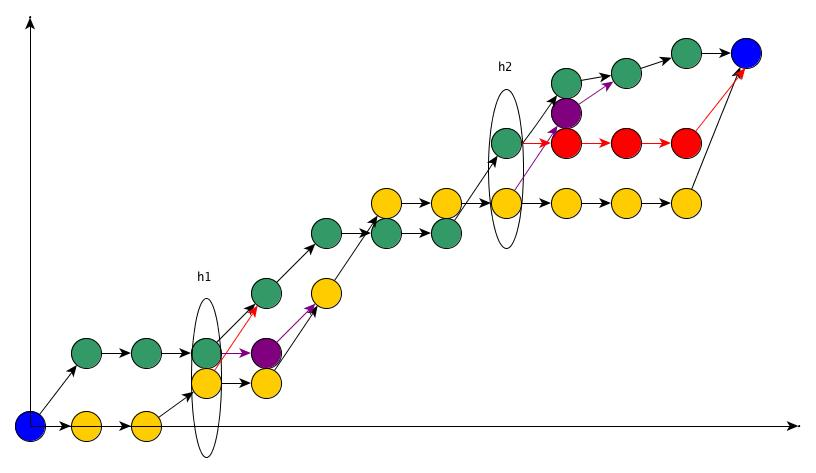
\includegraphics[scale=0.4]{images/croisementADG.jpg}
\end{center}
 On remarque qu'avec l'utilisation de l'évalution incrémentale, seuls deux arcs sont à réévaluer à chaque fois, car les arcs intermédiares correspondant à une quantité constante ont une évalution égale à zéro.
\subsection*{Mutation}
La mutation consiste à remplacer un sommet du chemin, par un sommet voisin. Par exemple sur ce shéma le sommet orange foncé serait remplacé par l'un des sommets orange clair.
\begin{center}
  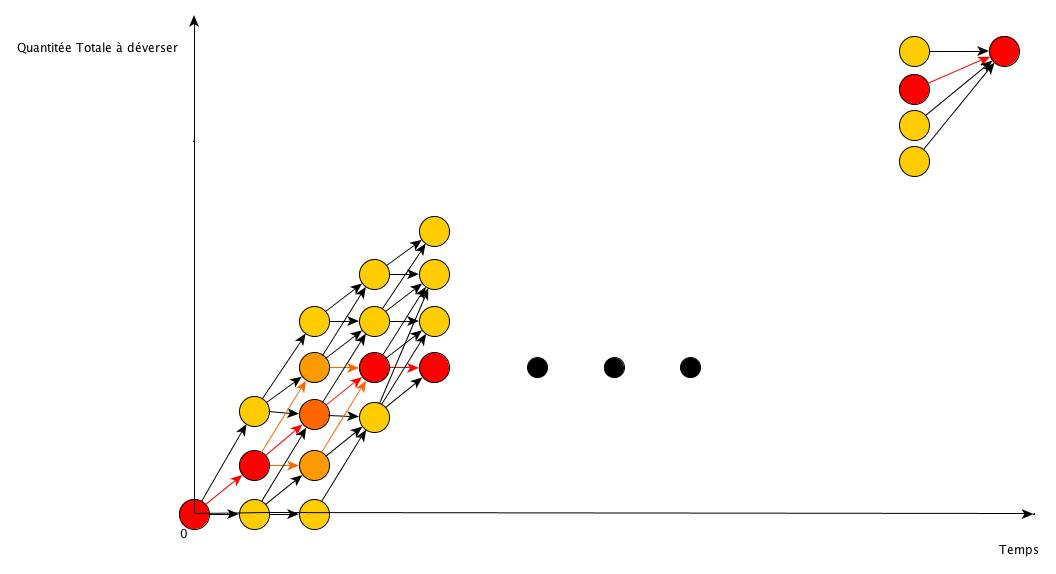
\includegraphics[scale=0.4]{images/mutationADG.jpg}
\end{center}
Nous avons fait le choix d'utiliser un pas de discrétisation variable pour le graphe, celui ci est donc fixé aléatoirement au début de la mutation entre une borne minimale et une borne maximale, qui peuvent être considérée comme des paramètres pour cette mutation. Le sommet muter est également choisi aléatoirement. On choisi ensuite de maniere aléatoire, si on remplace le sommet par le voisin correspondant pour le pas de discrétisation selectionné, à une quantité supérieure ou a une quantité inférieureion, c'est le sens de mutat. S'il n'est pas possible de muter dans le sens selectionné le sommet à muter, on essaie de muter dans l'autre sens, s'il n'est pas possible de muter le sommet selectionné dans quelque sens que ce soit, on en choisit aléatoirement un autre. On montre l'ergodicité de cette mutation (voire annexe), celà permet de nous assurer que tout individu soit mutable à partir du moment ou l'arbre obtenu avec le pas de discrétisation, possède plus qu'un seul et unique chemin.\\
Si l'on utilise l'évaluation incrémentale, il n'y a apres cette mutation que 2 arcs à réévaluer.
\subsection*{Mutation complémentaire}
Afin d'augmenter la vitesse de convergence on ajoute une seconde mutation. L'idée est de selectionner 2 heure éloigner de 24 heures, et de remplacer le chemin entre ces deux heures, par le chemin le plus long.
\begin{center}
  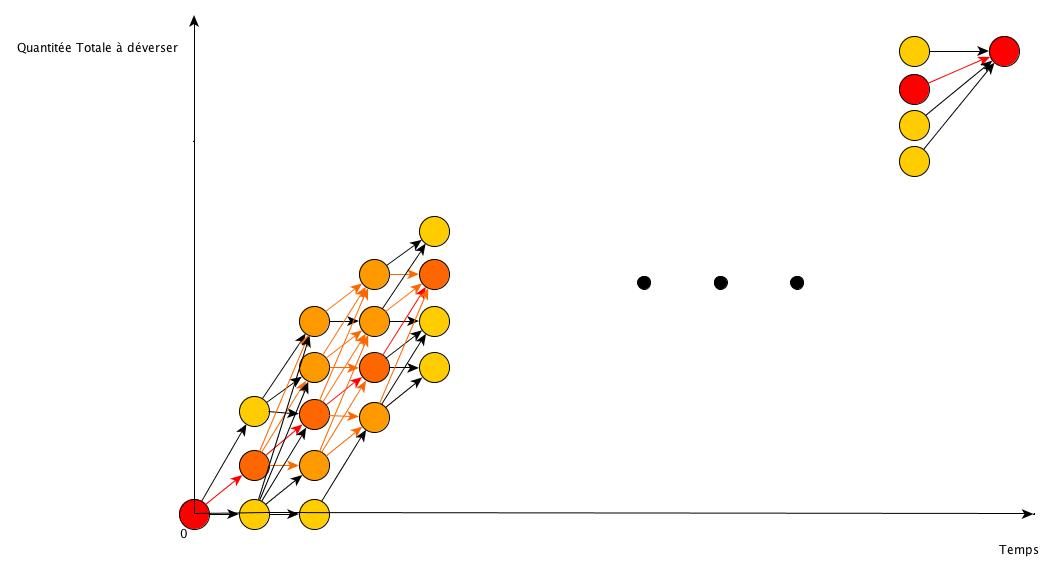
\includegraphics[scale=0.4]{images/mutationADG2.jpg}
\end{center}
Le plus long chemin entre les deux points selectionnés est trouvé de par un MIP grace à cplex.
\subsection*{Evaluation}
L'évaluation consiste à évaluer chaque arcs constituant le chemin et à les sommer. Pour se faire on va utiliser une fonction de decodage :
\begin{center}
  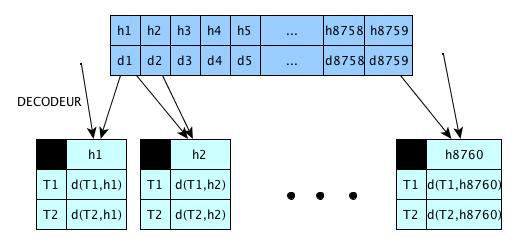
\includegraphics[scale=0.5]{images/representionADG.jpg}
\end{center} 
Le décodage utilise la programmation linéaire en variable mixte avec cplex. Qui plus est on utilise l'évaluation incrémentale, c'est à dire que l'on ne réévalue que les arcs pour lesquels la quantité à distribuer à été modifié par l'un des opérateurs de croisement ou de mutation.
\subsection{Résultats}
\subsubsection*{Premier paramétrage}
Les premiers tests ont été effectués sur une population de 100 individus, avec elitisme. La probabilité qu'il y ait une mutation est de 0.1 et lorsqu'un individu est muté la probabilité qu'il subisse la premiere mutation est de 100$\%$ ainsi que celle qu'il subisse la deuxième mutation.\\
\begin{center}
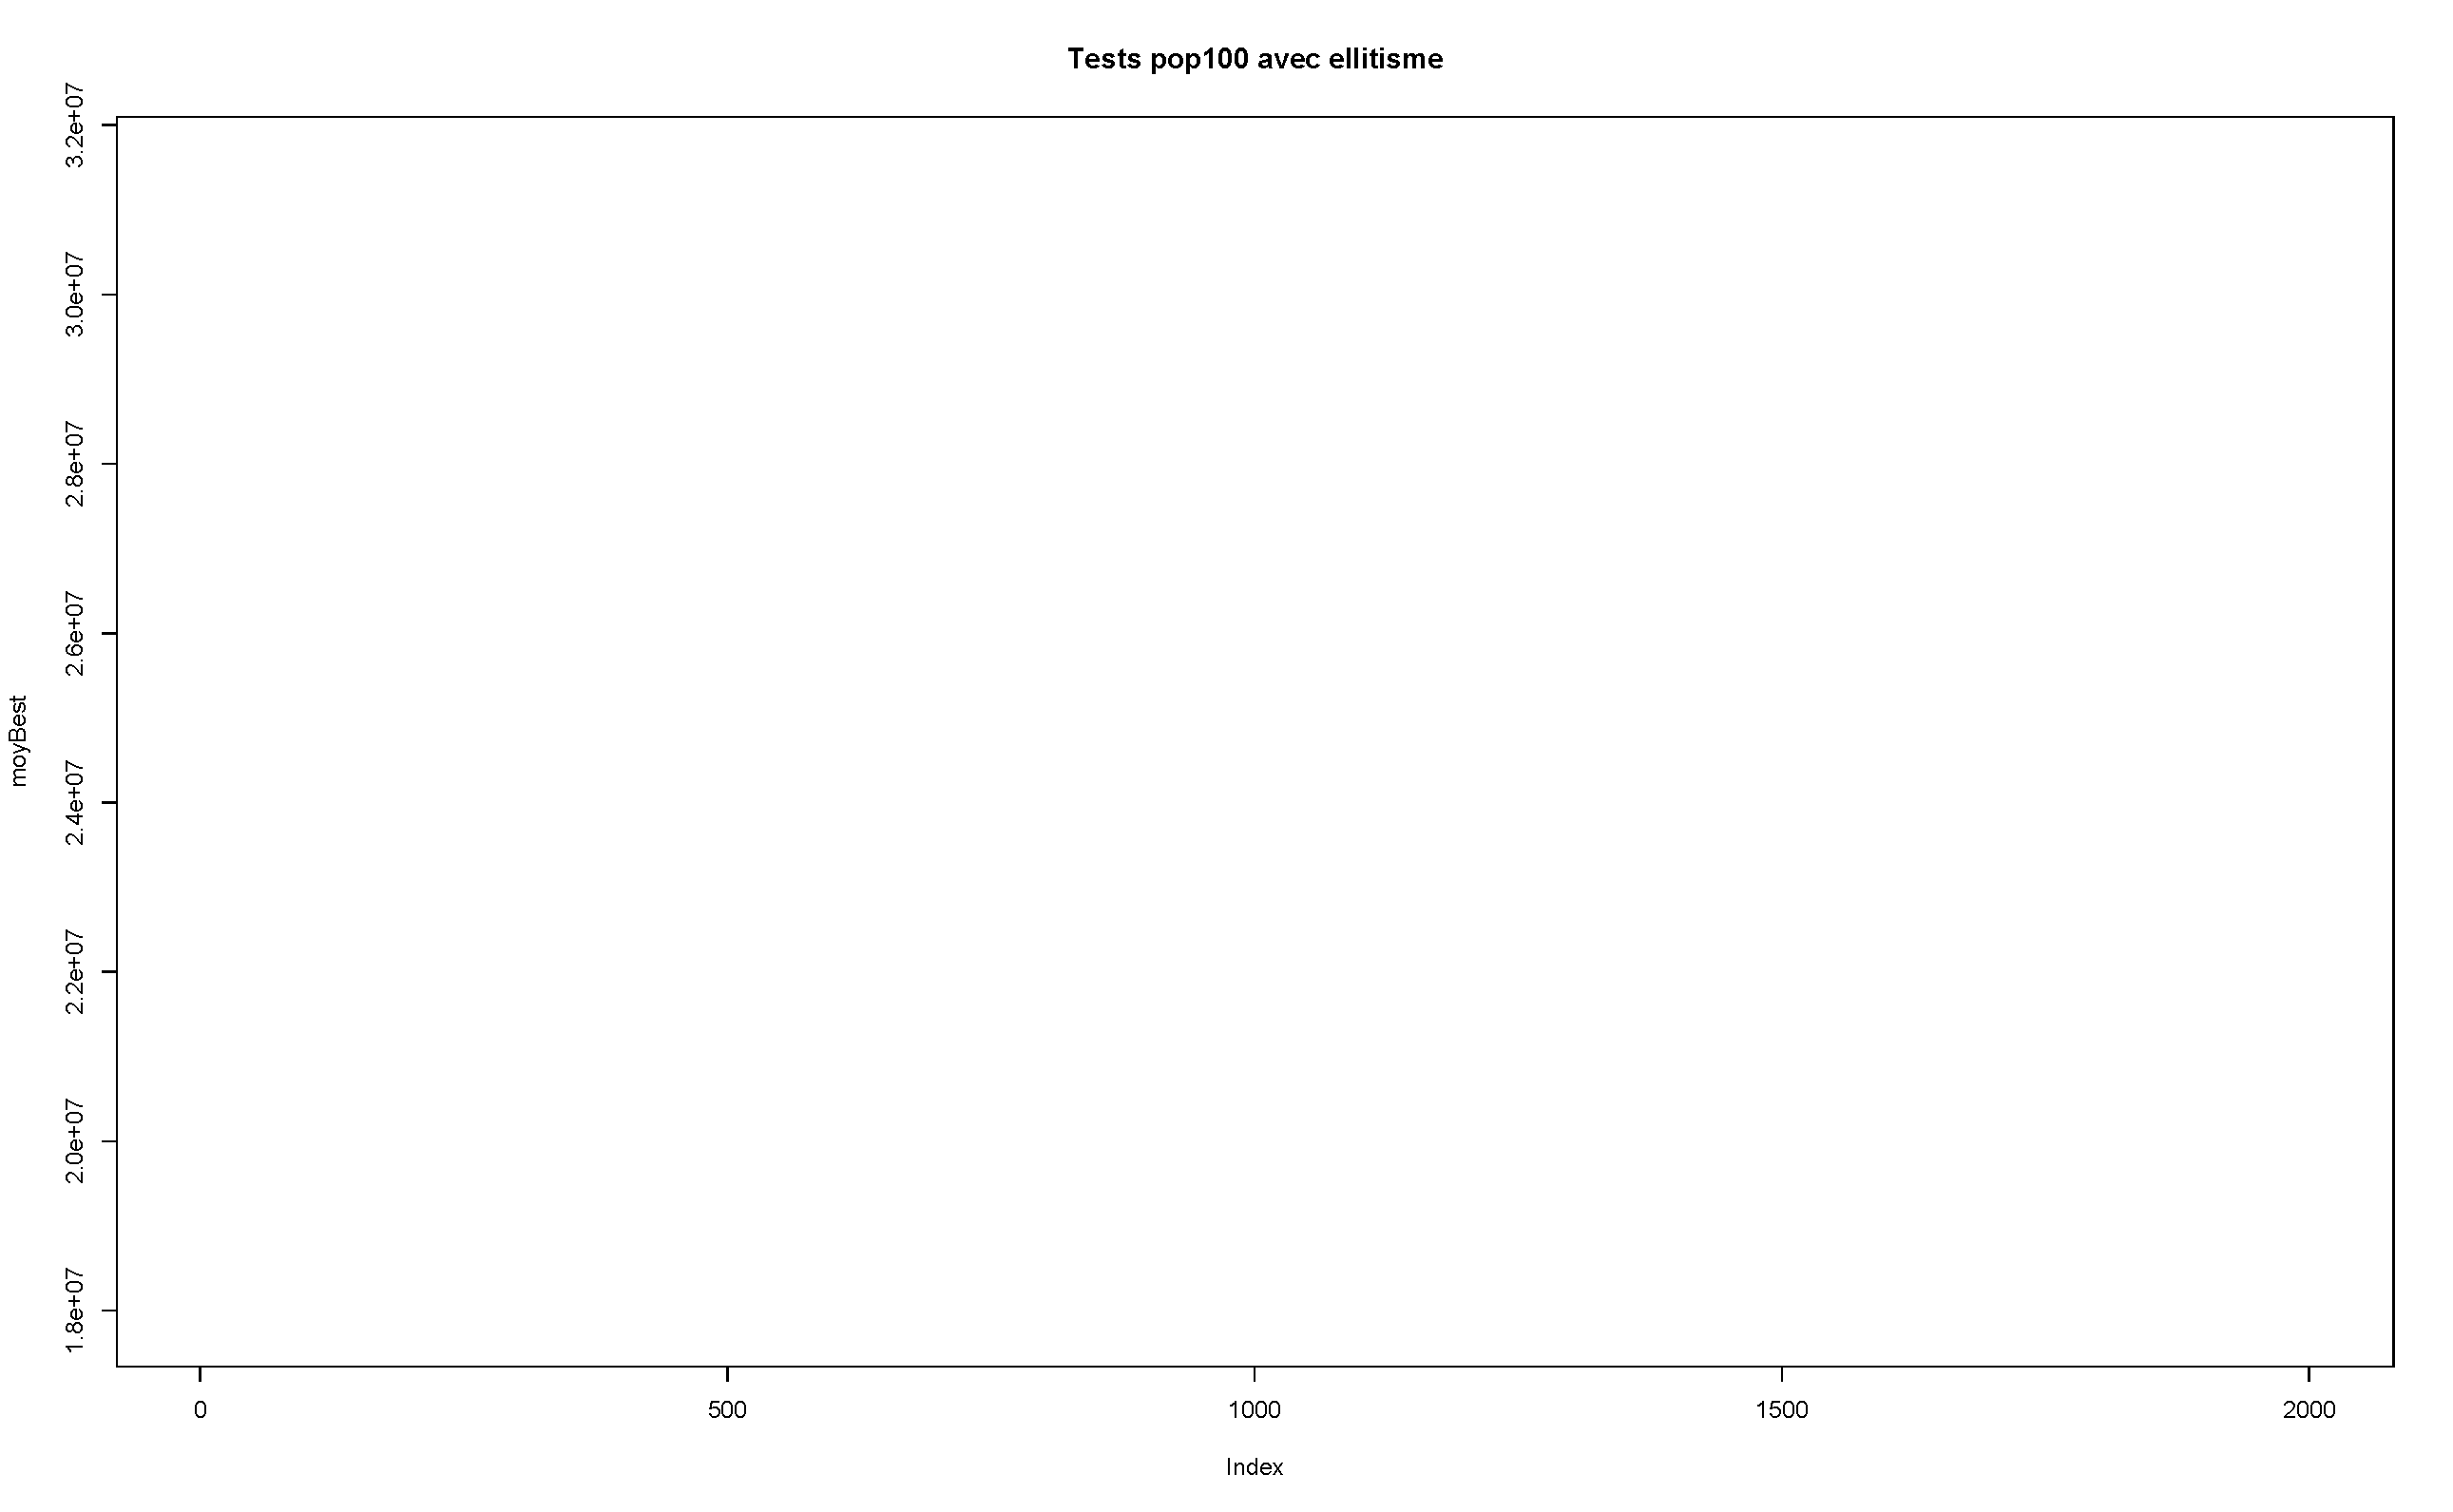
\includegraphics[scale=0.3]{images/test1.pdf}
\end{center}
Ce graphique montre en rouge l'évolution moyenne ( sur un ecantillon de 20 tests) de la  meilleure solution trouvée par l'algorithme en fonction du nombre de génération. Et en noir l'évolution de la valeur moyenne de la population. On peut observer que la population reste peu diversifier c'est pourquoi nous allons faire d'autres tests en faisant varier les parametres de mutation.\\
\subsubsection*{Deuxième paramétrage}
\subsubsection*{Troisième paramétrage}
\subsubsection*{Quatrième paramétrage}
\subsection{Idées et perspectives}
\begin{itemize}
  \item Delta-évaluation: Au lieu de sommer à chaque fois 8760 valeurs, on calcul:
  \begin{center}
     $eval= eval + \sum_{a \in ArcsModifiés} nouvelleEval_a - \sum_{a \in ArcsModifiés} ancienneEval_a$
    
  \end{center}
  \item Mettre en oeuvre l'idée d'amélioration sur l'initialisation.
  \item Tester d'autres stratégies de selection ou/et de remplacement
  \item combiner avec l'idée de décompopsition spaciale en ne prenant pour individus une liste de sommets du graphe tous disjoint de 24h (par exemple), et en considérant que les chemins liant ses différents sommets sont à chaque fois les chemins de longueur maximale.
  
  \item Utiliser des individus qui reprèsentent des portions de graphes et non de simple chemins ...
  
\end{itemize}
\chapter{Comparaison des différentes méthodes}


\end{document}
